\documentclass{article}


\usepackage[utf8]{inputenc}		% for special characters
\usepackage[english]{babel}
%\usepackage[T1]{fontenc}		% for correct use of western european characterfonts
\usepackage{amsmath}
\usepackage{bm}
\usepackage{natbib}
\usepackage{amssymb}
\usepackage{bbm}

\usepackage{titling}


\usepackage{graphicx}


\usepackage{algorithm}
\usepackage{algpseudocode}
% \usepackage{algorithm}
% keine "End"-Statements in Algorithmen
\algtext*{EndWhile}
\algtext*{EndIf}
\algtext*{EndFor}
\algtext*{EndProcedure}
\algtext*{EndFunction}



\usepackage{caption}
\DeclareCaptionType{code}[Code Listing][List of Code Listings] 

\usepackage{listings}
\usepackage{color}
\definecolor{matlabgreen}{RGB}{28,172,0}
\definecolor{matlabpurple}{RGB}{170,55,241}	
	
\lstset{language=Matlab,
	breaklines=true,
	keywordstyle=\color{blue},
	identifierstyle=\color{black},
	stringstyle=\color{matlabpurple},
	commentstyle=\color{matlabgreen},
	showstringspaces=false,
	numbers=left,
	numberstyle={\color{black}},
	numbersep=9pt
}



\newcommand{\norm}[1]{\left\lVert#1\right\rVert}


\setlength{\parskip}{\baselineskip}
%\setlength{\parindent}{0pt}%

%\setlength{\parindent}{2em}
%\setlength{\parskip}{1em}
%\renewcommand{\baselinestretch}{1.5}


\begin{document}

\title{Kernel Density Estimates and Mean Shift Clustering}
\author{Jonas Spinner\thanks{jonas.spinner@student.kit.edu} \enspace -- 1927895\\
	Analytics and Statistics\\
	KIT -- Karlsruhe Institute of Technology}
\date{January 21, 2019}
\maketitle

\newpage

\tableofcontents

\newpage

\listoffigures

\listoftables

\listofalgorithms

\listofcodes


\newpage


\begin{abstract}
	In this seminar paper we are describing and evaluating the mean shift algorithm. It is a nonparametric clustering method which does not depend on prior knowledge of the number and shape of the clusters.
	
	The clusters are defined by the modes of the data density and an iteration procedure is used to let a point converge to its cluster centroid. We introduce the kernel density estimate for estimating the data density and then derive the mean shift algorithm from it.
	
	After presenting the methods we also present different applications of the algorithm, primarily the use in image segmentation.
\end{abstract}

\section{Introduction}

In this seminar paper we are going to discuss the method of kernel density estimation and its use in the mean shift clustering algorithm. Clustering is one of the main tasks in machine learning and the mean shift algorithm has many applications, mainly in computer vision tasks. The mean shift algorithm is a nonparametric approach which allows a wide range of data distributions without imposing any prior knowledge.

The content of this seminar paper is mainly based on \cite{Comaniciu.2002}. First, we introduce the kernel density estimate in section \ref{sec:kernel-density-estimation}. In section \ref{sec:mean-shift-clustering} we derive the mean shift algorithm by estimating the density gradient. Then we finally state the mean shift algorithm. In section \ref{sec:application} we look at applications of the algorithm and describe our implementation in Matlab.

\textbf{History}

The mean shift algorithm was introduced in \cite{Fukunaga.1975} where also the term ``mean shift'' was established. Later \cite{Comaniciu.2002} and \cite{Comaniciu.2003} are responsible for a gain in interest for the algorithm. These publications popularized the use of the algorithm in image segmentation, image filtering and  object tracking.


\textbf{Notation}

In this paper we use the following conventions. Bold symbols like $\bm{x}$ denote a vector or a vector valued function like $\bm{m}(\cdot)$. $\{ \bm{x}_i \}_{i=1}^n$ denotes the set with $n$ samples $\bm{x}_i$, indexed by $i$. Throughout the seminar paper $d$ is the dimension of the samples. Upper case functions like $K(\cdot)$ denote a multivariate kernel function $\mathbb{R}^d \rightarrow \mathbb{R}$ and $k(\cdot)$ denotes a univariate function $[0, \infty) \rightarrow [0, \infty)$.


\section{Kernel Density Estimation} \label{sec:kernel-density-estimation}

In this section we are going to introduce the kernel density estimate. It is the main concept behind the mean shift algorithm and will be used in its derivation.

We assume that we have $n$ data points $\{\bm{x}_i\}_{i=1}^n \subset \mathbb{R}^d$, which are independently, identically distributed samples from an unknown distribution with the probability density function $f(\bm{x})$. The goal of density estimation is to estimate $f(\bm{x})$.

% Histograms estimate the probability distribution by bucketing the samples and counting the proportion of samples which fall in each bucket.

The \textbf{kernel density estimate} is defined as
\begin{equation}
	\hat{f}(\bm{x}) = \frac{1}{nh^d} \sum_{i=1}^n K\left(\frac{\bm{x} - \bm{x}_i}{h} \right) \qquad \bm{x} \in \mathbb{R}^d\text{,}
	\label{eq:kernel-density-estimate}
\end{equation}
where $n$ is the sample size, $d$ is the dimensionality of the data, $K(\bm{x})$ is a kernel function and $h$ is a bandwidth parameter. The estimate is dependent on the choice of the kernel function and the bandwidth.

A \textbf{kernel function} $K(\bm{x})$ is a function that satisfies
\begin{equation}
	K(\bm{x}) \geq 0\quad \text{and}\quad \int_{\mathbb{R}^d} K(\bm{x}) d\bm{x} = 1\text{.}
\end{equation}
These restrictions on the kernel ensure that $\hat{f}(\bm{x})$ is a valid density.

The \textbf{bandwidth} $h$ controls the smoothness of the kernel density estimate. The choices for kernel functions and the bandwidth are going to be discussed in section \ref{sec:popular-kernels} and section \ref{sec:bandwidth-selection}.

The kernel density estimate can be interpreted as the sum of ``bumps'' centered on each data point. In Figure \ref{fig:kde-kernel-density-estimates} the process of kernel density estimates is illustrated. The original density function is estimated based on five samples. For density estimation three methods are compared: a histogram, a kernel density estimate with a uniform kernel and a kernel density estimate with a gaussian kernel.

\begin{figure}
	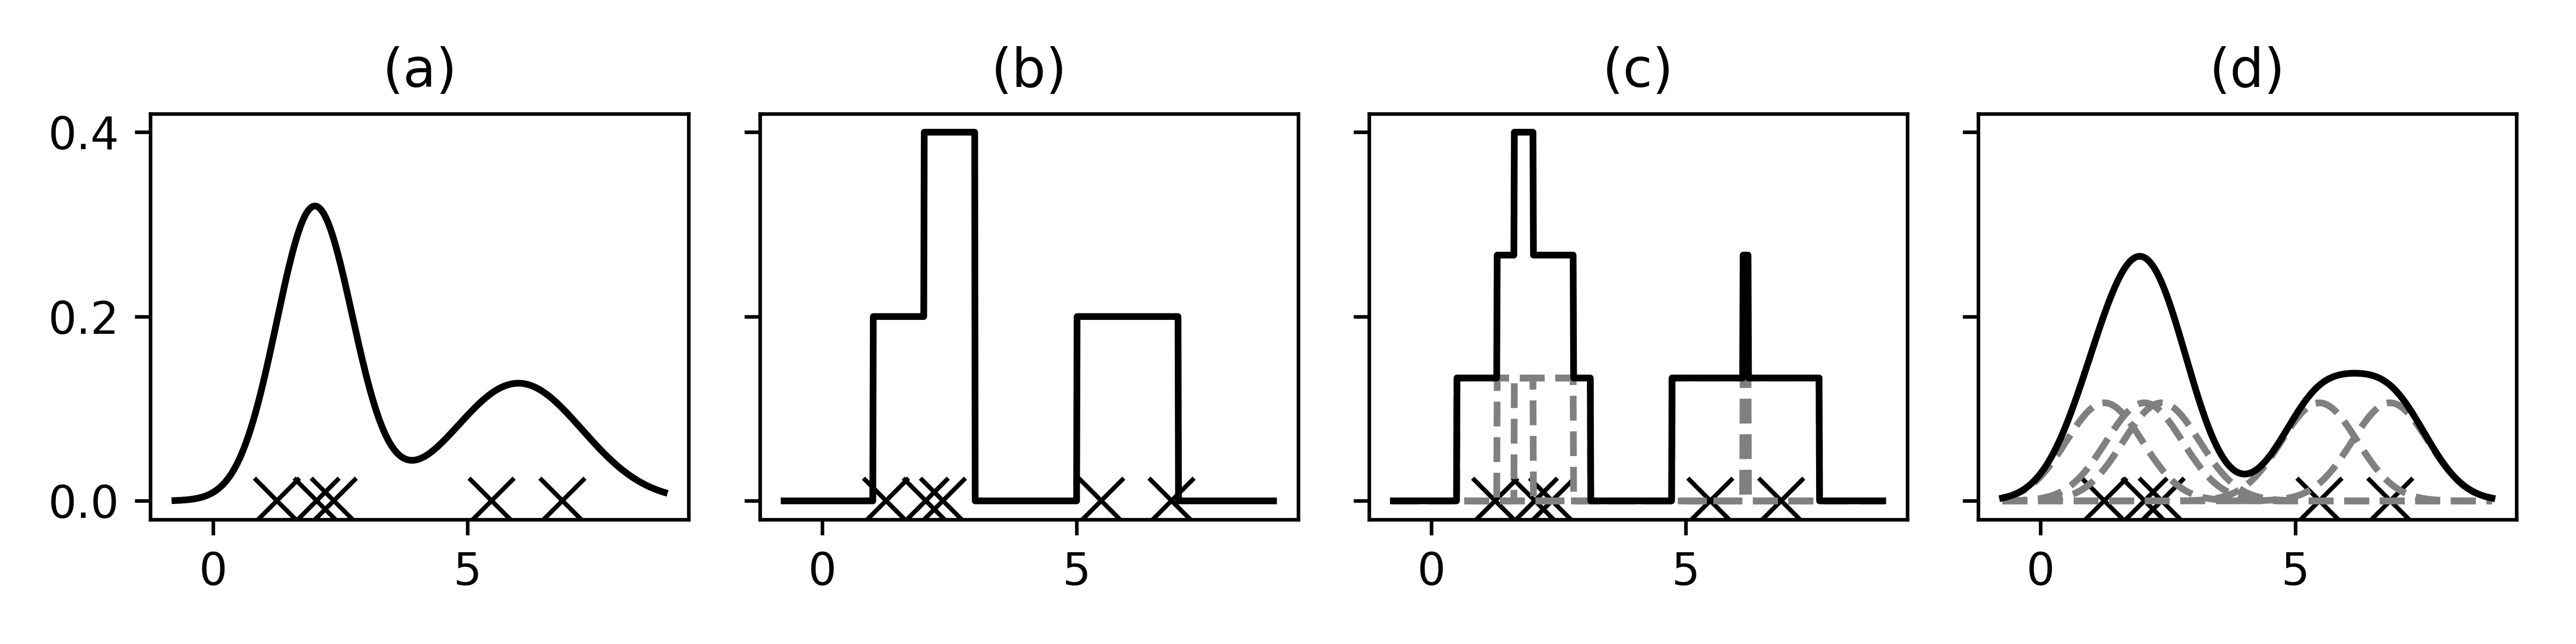
\includegraphics[width=\textwidth]{figures/kde-kernel-density-estimates}
	\caption[Samples, histogram and kernel density estimates]{Samples, histogram and kernel density estimates. Author's illustration.
		(a) The probability density distribution $\frac{3}{5} \mathcal{N}\left(2, 0.75^2\right) + \frac{2}{5} \mathcal{N}\left(6, 1.25^2\right)$ and five samples drawn from it.
		(b) A histogram with bins $[i,i+1)$, $i \in \mathbb{Z}$.
		(c) A kernel density estimate with a uniform kernel and bandwidth $h=0.75$, $K(x) = \frac{1}{2h}$ for $\lvert x \rvert \leq h$ and $0$ else.
		(d) A kernel density estimate with a gaussian kernel and bandwidth $h=0.75$, $K(x) = \frac{1}{h} \frac{1}{\sqrt{2\pi}} \exp(-\frac{1}{2} \lvert \frac{x}{h} \rvert^2)$.
	}
	\label{fig:kde-kernel-density-estimates}
\end{figure}


%\subsection{Other methods}

%Another method for estimating a probability density function are histograms. The samples $\{ \bm{x}_i \}_{i=1}^n$ are put into distinct buckets $b_j \subseteq \mathbb{R}^d$ and the probability is estimated by the sample frequency $p(j) = \lvert \{\bm{x}_i \mid \bm{x}_i \in b_j\} / n$ for each bucket.


\subsection{Popular Kernels} \label{sec:popular-kernels}

In this section we are going to present popular kernel functions and introduce the concept of radially symmetric kernels. This class of kernels is useful in the derivation of the mean shift algorithm.

\begin{figure}
	\centering
	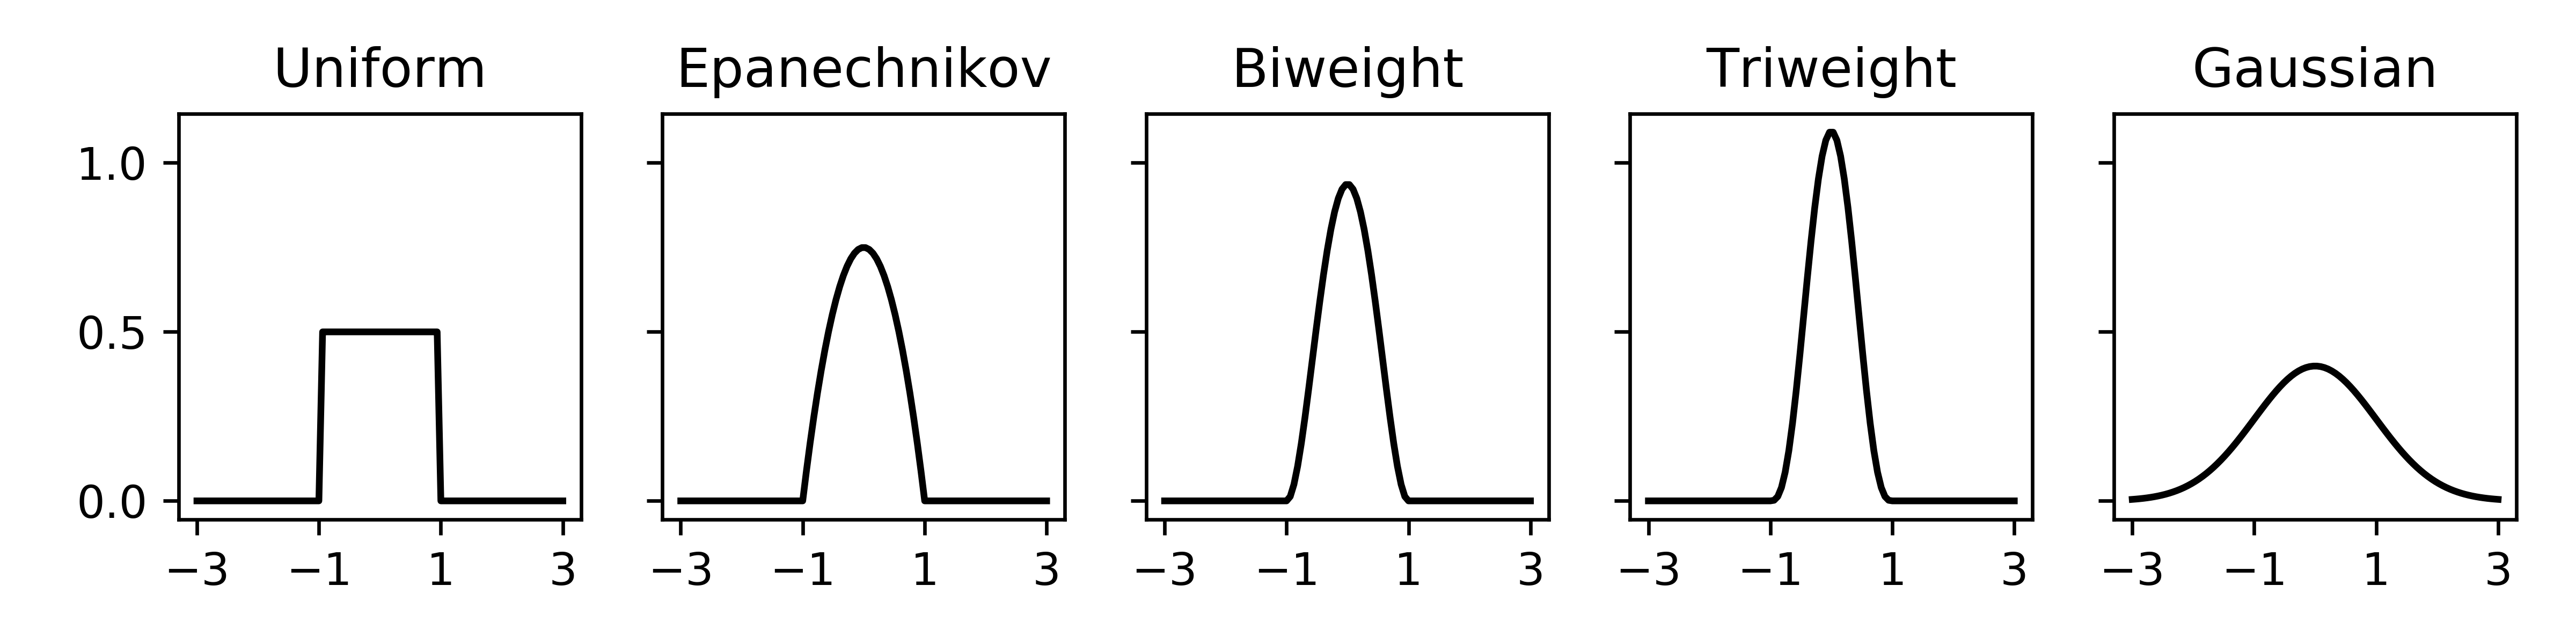
\includegraphics[width=\textwidth]{figures/kde-popular-kernels}
	\caption[Popular kernels]{Popular kernels. Author's illustration. The function definitions are listed in Table \ref{tab:popular-kernel-functions}. The first four kernels all have support $[-1, 1]$. The gaussian kernel has the support $(-\infty, \infty)$.}
	\label{fig:kde-popular-kernels}
\end{figure}

\newpage
\textbf{Radially symmetric kernels} are kernel functions which can be formulated as
\begin{equation}
	K(\bm{x}) = c_{k,d} k(\norm{\bm{x}}^2)\text{,}
\end{equation}
where $k : [0, \infty) \rightarrow [0, \infty)$ is called the \textbf{profile} of $K$, and $c_{k,d}$ is a constant which ensures, that $K(\cdot)$ integrate to 1.


The literature regarding mean shift clustering only uses a few distinct kernels. The most popular kernels for mean shift clustering are the uniform, the Epanechnikov and the gaussian kernel which are all radially symmetric kernels. We are going to shortly introduce them and their profile.

The \textbf{uniform kernel} is defined by being proportional to the indicator function of the unit hypersphere and can be written as
\begin{equation}
	K_U(\bm{x}) = \begin{cases}
		\text{vol}(S_d)^{-1} & \text{for} \norm{\bm{x}} \leq 1\\
		0 & \text{else}
	\end{cases}\text{,}
\end{equation}
where $\text{vol}(S_d) = \pi^{d/2}\Gamma((d+2)/2)^{-1}$ is the volume of the $d$-dimensional hypersphere with $\Gamma(\cdot)$ being the gamma function. For $d=1$ the volume $\text{vol}(S_d)$ equals 2. The corresponding profile $k_U$ is
\begin{equation}
	k_U(u) = \begin{cases}
		1 & \text{for } 0 \leq u \leq 1\\
		0 & \text{for } 1 < u\text{.}
	\end{cases}
\end{equation}

The \textbf{Epanechnikov kernel} is defined as
\begin{equation}
	K_E(\bm{x}) = \begin{cases}
		\frac{2 + d}{2 \text{vol}(S_d)} (1 - \norm{\bm{x}}^2) & \text{for } \norm{\bm{x}} \leq 1\\
		0 & \text{else}
	\end{cases}
\end{equation}
and its profile $k_E$ is
\begin{equation}
	k_E(u) = \begin{cases}
		1 - u & \text{for } 0 \leq u \leq 1\\
		0 & \text{for } 1 < u\text{.}
	\end{cases}
\end{equation}
The Epanechnikov kernel is an optimal kernel in the sense that it minimizes the quality measure AMISE\footnote{AMISE stands for approximation of the mean square error between the density and the estimate integrated over the domain \citep[p. 5]{Comaniciu.2002}.}.

The \textbf{gaussian kernel} is defined as
\begin{equation}
	K_G(\bm{x}) = (2 \pi)^{-d/2} \exp\left(-\frac{1}{2} \norm{\bm{x}}^2\right)
\end{equation}
and its profile $k_G$ is
\begin{equation}
	k_G(u) = \exp\left(-\frac{1}{2}u\right)\text{.}
\end{equation}
The gaussian kernel is one of the few kernels which has a non-compact support. That can pose a problem because every point $\bm{x}\in\mathbb{R}$ gets assigned a non-zero weight $K_G(\bm{x})$. In practical applications the kernel is often truncated, and the very small weights are ignored.

We present the kernels, their support and profile in Table \ref{tab:popular-kernel-functions} for future reference. 

\begin{table}
	\begin{center}
		\begin{tabular}{r|r|r|r|l}
			\textbf{Name} & \textbf{Profile support} & $k(u)$ & $-k'(u)$ & $K(\bm{x})$ \\ \hline\hline
			Uniform & $u \in [0, 1]$ & $1$ & $0$ & $\text{vol}\left(S_d\right)^{-1}$ \\
			Epanechnikov & $u \in [0, 1]$ & $1 - u$ & $1$ & $\frac{1}{2} \text{vol}(S_d)^{-1} (d+2) \left(1 - \norm{\bm{x}}^2\right)$\\
			Biweight & $u \in [0, 1]$ & $(1 - u)^2$ & $2 (1 - u)$ & $\propto \left(1 - \norm{\bm{x}}^2\right)^2$ \\
			Triweight & $u \in [0, 1]$ & $(1 - u)^3$ & $3 (1 - u)^2$ & $\propto \left(1 - \norm{\bm{x}}^2\right)^3$ \\
			Gaussian & $u \in [0, \infty)$ & $\exp\left(-\frac{1}{2}u\right)$ & $\frac{1}{2}\exp\left(-\frac{1}{2}u\right)$ & $(2\pi)^{-d/2} \exp\left(-\frac{1}{2}\norm{\bm{x}}^2\right)$
		\end{tabular}
	\end{center}
	\caption[Popular kernel functions]{Popular kernel functions. The kernel functions listed here are all radially symmetric kernels. By looking at the profiles $k(u)$ and the negated derivative $-k'(u)$ we can see the corresponding shadows (see section \ref{sec:mean-shift-vector-properties}). $\text{vol}(S_d)$ is the volume of a $d$-dimensional hypersphere and the normalization constants for the biweight and triweight kernels are omitted.}
	\label{tab:popular-kernel-functions}
\end{table}


\subsection{Bandwidth Selection} \label{sec:bandwidth-selection}

One of the main challenges in using the kernel density estimate in practice is the choice of the bandwidth. The univariate case has a rich theoretical background and many ``rule of thumbs'' are formulated, but the multivariate case lacks those. In \citep[section 3.1]{Comaniciu.2002} some general approaches for bandwidth selection are listed.

\begin{itemize}
	\item The stability of the clustering in respect to the bandwidth parameter $h$ is analyzed. The number of resulting clusters $K$ is stated as a function of the bandwidth, $K(h)$. Then the midpoint of the largest range for which $K(h)$ stays constant is chosen.
	\item Some objective function is used for evaluating the clustering quality. The bandwidth which maximizes the objective function is chosen.
	\item When the desired number of clusters is known, the bandwidth can be varied to accomplish the desired number. This approach can be modified to ignore smaller clusters.
	\item Another approach is to estimate the bandwidth by the mean $K$ nearest neighbor distance between the data points. $K$ is set to be a percentage of the whole dataset, for example 30 \%.
\end{itemize}

More bandwidth selection techniques are proposed in the literature but are not covered by us.

For our seminar paper we are implemented the $K$ nearest neighbor approach. The Python library scikit-learn from \cite{Pedregosa.2011} implements this approach as \texttt{estimate\_bandwidth}. Our code can be found in Code Listing \ref{code:estimate_bandwidth}.

%\begin{equation}
%\hat{f}_{-i}(\bm{x}) = \frac{1}{(n - 1)h^d} \sum_{j \neq j} K\left(\frac{\bm{x}_j - \bm{x}_j}{h} \right) \qquad \bm{x} \in \mathbb{R}^d
%\end{equation}
%
%\begin{align}
%\text{MLCV}(h) &= \frac{1}{n} \sum_{i=1}^n \log \hat{f}_{-i}(\bm{x}_i) \\
%&= \frac{1}{n} \sum_{i=1}^n \log \left(\sum_{j \neq j}^n K\left(\frac{\bm{x}_j - \bm{x}_j}{h} \right)\right) - \log(n - 1) - d \log(h)
%\end{align}



\section{Mean Shift Clustering} \label{sec:mean-shift-clustering}

In this section we are going to give a general overview of the clustering task and different clustering algorithms in section \ref{sec:clustering-algorithms}. Then we will look at density gradient estimation in section \ref{sec:density-gradient-estimation} and derive properties of the mean shift vector. Equipped with these perquisites we are formulate the mean shift algorithm in section \ref{sec:mean-shift-algorithm}.

Clustering is one of the main machine learning tasks, concerned with grouping objects $\{x_i\}_{i=1}^n$ into clusters $C_j$ resulting in a clustering $\mathcal{C} = \{ C_j \}_{j=1}^K$.

\subsection{Clustering algorithms} \label{sec:clustering-algorithms}

What does define a ``good'' clustering? One can try to minimize a global criterion. For example the $K$-Means algorithm tries to minimize the intra cluster variance $J = \sum_{j=1}^K \sum_{\bm{x}_i \in C_j} \norm{\bm{x}_i - \bm{m}_j}^2$ and hierarchical clustering minimizes the intra-cluster min, max or average distances between the data points. The notion of a ``good'' clustering brings rise to many different clustering algorithms.

Other criteria to differentiate clustering algorithms, are the assumptions that it makes on the data. That can be the number and shapes of clusters, e.g. $K$-Means assumes the data is separable into $K$ clusters. 

\textbf{Centroid based algorithms}

A common concept for several algorithms is a \textbf{centroid}. A centroid is a point in the data space, which is a representative for a cluster. $K$-Means defines its centroids as the cluster means $\bm{m}_j = \lvert C_j \rvert^{-1} \sum_{\bm{x}_i \in C_j} \bm{x}_i$. A problem with this approach is that the cluster mean is not guaranteed to ``look like'' a typical data object, meaning that the centroid can lie in an environment with no real data points in its neighborhood.

``Low density centroids'' can be avoided by defining the centroids to be the \textbf{modes of the probability density function}. That's the core idea of the mean shift clustering algorithm. It estimates the underlying density of the data objects and searches for points which high relative probability. Or in other words it searches for the modes of the estimated density.

This approach has some nice benefits. The number of clusters is defined by the number of modes and clusters can have an arbitrary shape.

For the mode finding procedure we need to work with gradient of the density and find the points $\bm{x}$ where $\nabla f(\bm{x}) = 0$. In the next section we look at a method to approximate the density gradient. 


\subsection{Density gradient estimation} \label{sec:density-gradient-estimation}

Before we look at the specifics of the mean shift algorithm in section \ref{sec:mean-shift-algorithm}, we look at an estimation of the density gradient and derive the mean shift vector. This section is based on \cite{Comaniciu.2002} and follows its notation.

By defining clusters with the modes of a density function the clustering task becomes a mode finding task where we search for $\bm{x}$ where the density gradient is zero, $\nabla f(\bm{x}) = 0$. As we have no knowledge about the real density $f(\bm{x})$, we must use an estimate. Recall that the kernel density estimate is defined as
\begin{equation}
	\hat{f}(\bm{x}) = \frac{1}{nh^d} \sum_{i=1}^n K\left(\frac{\bm{x} - \bm{x}_i}{h} \right)\text{.}
\end{equation}

We estimate the density gradient $\nabla f(\bm{x})$ by the gradient of the density estimate:
\begin{equation}
	\hat\nabla f(\bm{x}) \equiv \nabla \hat{f}(\bm{x}) = \frac{1}{nh^d} \sum_{i=1}^n \nabla K\left(\frac{\bm{x} - \bm{x}_i}{h} \right)\text{.}
\end{equation}

For simplification we are going to concentrate on \textbf{radially symmetric kernels} that we have introduced in section \ref{sec:popular-kernels}. Recall that these kernels can be written as
\begin{equation}
	K(\bm{x}) = c_{k,d} k(\norm{\bm{x}}^2)
\end{equation}
where $k : [0, \infty]) \rightarrow [0, \infty)$ is called the \textbf{profile} of $K$, and $c_{k,d}$ is a constant which ensures that $K(\bm{x})$ integrate to $1$.

Because we are going to use different kernel density estimates, we now explicit state the used bandwidth $h$ and kernel $K$ of the kernel density estimate as $\hat{f}_{h,K}(\bm{x})$. The kernel density estimate can now be formulated as
\begin{equation}
	\hat{f}_{h,K}(\bm{x}) = \frac{c_{k,d}}{nh^d} \sum_{i=1}^n k\left(\norm{\frac{\bm{x} - \bm{x}_i}{h}}^2 \right)
\end{equation}
and its gradient as
\begin{equation}
	\nabla \hat{f}_{h,K}(\bm{x}) = \frac{2c_{k,d}}{nh^{d+2}} \sum_{i=1}^n (\bm{x} - \bm{x}_i)k'\left(\norm{\frac{\bm{x} - \bm{x}_i}{h}}^2 \right)\text{.}
\end{equation}

With the substitution $g(u) = -k'(u)$ and reordering, we can formulate the gradient as
\begin{equation}
	\nabla \hat{f}_{h,K}(\bm{x}) = \frac{2c_{k,d}}{nh^{d+2}} \left[\sum_{i=1}^n g\left(\norm{\frac{\bm{x} - \bm{x}_i}{h}}^2 \right)\right] \left[\frac{\sum_{i=1}^n \bm{x}_i g\left(\norm{\frac{\bm{x} - \bm{x}_i}{h}}^2 \right)}{\sum_{i=1}^n g\left(\norm{\frac{\bm{x} - \bm{x}_i}{h}}^2 \right)} - \bm{x}\right]\text{.}
	\label{equ:kde-gradient-3-terms}
\end{equation}

We can analyze the terms separately. The last term is called \textbf{mean shift vector}
\begin{equation}
	\bm{m}(\bm{x}) = \frac{\sum_{i=1}^n \bm{x}_i g\left(\norm{\frac{\bm{x} - \bm{x}_i}{h}}^2 \right)}{\sum_{i=1}^n g\left(\norm{\frac{\bm{x} - \bm{x}_i}{h}}^2 \right)} - \bm{x}\text{.}
\end{equation}

We introduced an estimate for the density gradient and the mean shift vector $\bm{m}(\bm{x})$. In section \ref{sec:mean-shift-vector-properties} we are going to further analyze the properties of $\bm{m}(\bm{x})$. In section \ref{sec:mean-shift-algorithm} we are finally presenting the mean shift algorithm and a short discussion follows in section \ref{sec:mean-shift-discussion}.


\subsection{Properties of the mean shift vector and kernel shadows} \label{sec:mean-shift-vector-properties}

We can further analyze the equation \ref{equ:kde-gradient-3-terms} and relate the mean shift vector to a kernel density estimate. The first two factors can be decomposed into a scaling factor and a kernel density estimate with the kernel $G(\bm{x}) = c_{g,d} g(\norm{\bm{x}}^2)$
\begin{align}
	\frac{2c_{k,d}}{nh^{d+2}} \left[\sum_{i=1}^n g\left(\norm{\frac{\bm{x} - \bm{x}_i}{h}}^2 \right)\right] &= \frac{2c_{k,d}}{h^2c_{g,d}} \left[\frac{c_{g,d}}{nh^d} \sum_{i=1}^n g\left(\norm{\frac{\bm{x} - \bm{x}_i}{h}}^2 \right) \right]\\
	&= \frac{2c_{k,d}}{h^2c_{g,d}} \hat{f}_{h,G}(\bm{x})\text{.}
\end{align}

With this formulation we can rewrite the density gradient estimate $\nabla \hat{f}_{h,K}(\bm{x})$ into
\begin{equation}
	\nabla \hat{f}_{h,K}(\bm{x}) = \frac{2c_{k,d}}{h^2c_{g,d}} \hat{f}_{h,G}(\bm{x}) \bm{m}(\bm{x})\text{.}
\end{equation}

That allows us to write the mean shift vector as a normalized gradient of the kernel density estimate $\hat{f}_{h,K}(\bm{x})$
\begin{equation}
	\bm{m}(x) = \frac{h^2c_{g,d}}{2c_{k,d}} \frac{\nabla \hat{f}_{h,K}(\bm{x})}{\hat{f}_{h,G}(\bm{x})}\text{.}
\end{equation}

We can observe that the mean shift vector calculated with the kernel $G$ points in the gradient direction of the kernel density estimate calculated with the kernel $K$.

\textbf{Shadows of kernels}

For the kernels $G(\bm{x}) \propto g(\norm{\bm{x}}^2)$ and $K(\bm{x}) \propto k(\norm{\bm{x}}^2)$, if $-k'(u) \propto g(u)$ then we call the kernel $K$ a \textbf{shadow} of kernel $G$.

The gaussian kernel is a shadow of itself. Recall that the profile of the gaussian kernel is $k_G(u) = \exp\left(-\frac{1}{2}u\right)$. It holds that $-k_G'(u) \propto k_G(u)$.

The Epanechnikov kernel is a shadow of the uniform kernel, because the profile of the Epanechnikov kernel is $k_E(u) = (1 - u) \mathbbm{1}\{u \in [0, 1]\}$ and $-k_E'(u) = k_U(u) = \mathbbm{1}\{u \in [0, 1]\}$.

%The mean shift vector $\bm{m}(\bm{x})$ calculated with the kernel $G$ is therefore not the gradient direction of a kernel density estimate calculated with $G$, but of the kernel density estimate calculated with a more ``complex'' kernel, the shadow of $G$.

% The mean shift vector $\bm{m}(\bm{x})$ inhibits some nice properties that makes it easy to compute. In section \ref{sec:kernel-density-estimation} we required that the kernel must integrate to $1$. This requirement can be dropped because the normalizing constants cancel in the expression.



\subsection{The mean shift algorithm} \label{sec:mean-shift-algorithm}

With the previously introduced concepts the mean shift algorithm can be quickly stated. Recall that the mean shift vector is
\begin{equation}
\bm{m}(\bm{x}) = \frac{\sum_{i=1}^n \bm{x}_i g\left(\norm{\frac{\bm{x} - \bm{x}_i}{h}}^2 \right)}{\sum_{i=1}^n g\left(\norm{\frac{\bm{x} - \bm{x}_i}{h}}^2 \right)} - \bm{x}\text{.}
\end{equation}

For each $\bm{x}_i$ we perform the iterative procedure
\begin{equation}
\bm{x}^{(t+1)} = \bm{x}^{(t)} + \bm{m}\left(\bm{x}^{(t)}\right)\text{,}\qquad t = 1, 2, ...
\end{equation}
where $\bm{x}^{(1)} = \bm{x}_i$. The procedure is stopped when $\bm{x}^{(t)}$ converges or at least the difference $\norm{\bm{x}^{(t+1)} - \bm{x}^{(t)}}$ is small enough. $\bm{z}_i$ gets assigned the value $\bm{x}^{(t)}$ is converged to.

After calculating $\bm{z}_i$ for each $\bm{x}_i$, the points for which $\bm{z}_i = \bm{z}_j$ are assigned to the same cluster. As before we relax this by assigning the same cluster when $\norm{\bm{z}_i - \bm{x}_j} < \varepsilon$ holds.

The mean shift algorithm is formulated in pseudo code as Algorithm \ref{alg:mean-shift-algorithm}.
\begin{algorithm}
	\begin{algorithmic}[1]
		\Function{MeanShift}{$\bm{x}_1, ..., \bm{x}_n : \mathbb{R}^d$, $h : \mathbb{R}^+$, $\varepsilon : \mathbb{R}^+$}
		\For{$i = 1..n$}
			\State $\bm{x}^{(1)} = \bm{x}_i$, $t=0$
			\Repeat
				\State $t = t + 1$
				\State $\forall j: w_j = \exp(-\frac{1}{2} \norm{(\bm{x}^{(t)} - \bm{x}_j) / h}^2)$
				\State $\bm{x}^{(t+1)} = (\sum_{j=1}^n w_j)^{-1} \sum_{j=1}^n w_j \bm{x}_j$
			\Until{$\norm{\bm{x}^{(t+1)} - \bm{x}^{(t)}} < tol$}
			\State $\bm{z}_i = \bm{x}^{(t+1)}$
		\EndFor
		\State \Return \Call{ConnectedComponents}{$\{\bm{z}_i\}_{i=1}^n, \varepsilon$}
		\EndFunction
	\end{algorithmic}
	\caption[Mean shift algorithm]{The mean shift algorithm with a gaussian kernel.}
	\label{alg:mean-shift-algorithm}
\end{algorithm}

\textbf{Convergence}

For the uniform kernel, the procedure is guaranteed to converge. For the samples $D = \{\bm{x}_i\}_{i=1}^n$ the number of weighted means of the subsets $D' \subseteq D$ is $2^n$. Each iterate $\bm{x}^{(t)}$ converges after finitely many steps.

The mean shift trajectories are illustrated in Figure \ref{fig:mean-shift-trajectories}. The dataset is a mixture of two gaussian distributions and the paths $\bm{x}^{(t)}$ are plotted. One can see that the trajectories of the data points meet at the two modes.

\begin{figure}
	\centering
	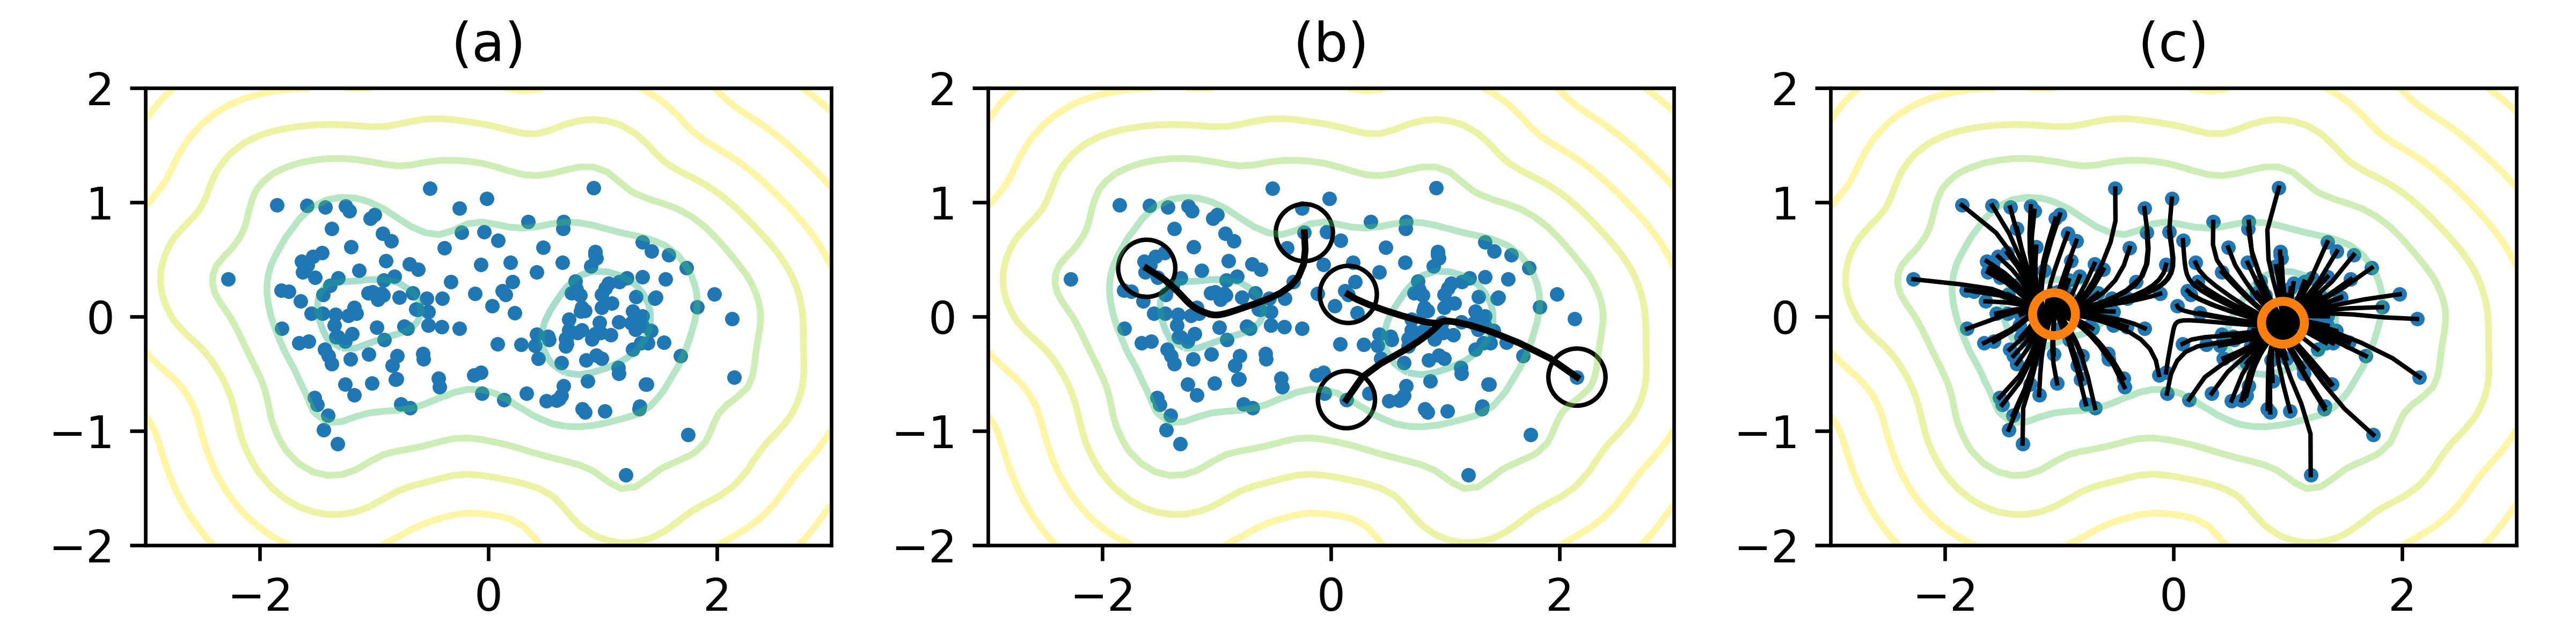
\includegraphics[width=\textwidth]{figures/mean-shift-trajectories.png}
	\caption[Mean shift trajectories]{Mean shift trajectories. Author's illustration. (a) The dataset is sampled from $\frac{1}{2} \mathcal{N}\left((1, 0)^T, 0.5^2\right) + \frac{1}{2} \mathcal{N}\left((-1, 0)^T, 0.5^2\right)$. The contour lines of $\log \hat{f}(\bm{x})$ are plotted. (b) The trajectories $\bm{x}^{(t)}$ for selected data points are plotted. A gaussian kernel was used with the bandwidth $h=0.25$. The circles are representing the bandwidth. (c) Trajectories for all data points. The cluster centroids are marked with  orange circles.}
	\label{fig:mean-shift-trajectories}
\end{figure}



\subsection{Discussion} \label{sec:mean-shift-discussion}

The mean shift algorithm has several advantages and disadvantages compared to other clustering algorithms. We are going to present possible solutions for some of them. This section is mainly based on \cite{CarreiraPerpinan.2015}.

\textbf{Advantages}

\begin{itemize}
	\item One of the main benefits is that the algorithm makes no prior assumptions about the number and shape of the clusters. This allows complex clusters with non-convex shapes.
	
	\item Outliers do not affect the clustering of the other data points. As outliers lie in low density regions their weight assigned by the kernel is either zero or very small.
	
	\item The algorithm only has one parameter, the bandwidth. The bandwidth has a easily understood interpretation and determines the resulting cluster uniquely. That can be used to formulate functions dependent on the bandwidth, e.g. some clustering criteria (see section \ref{sec:bandwidth-selection}).
	
	\item The cluster centroids can be interpreted as the modes of the estimated density function. That has the benefit that, ignoring the outliers, the centroids are ``typical'' data objects in that they are from a locally high-density environment.
\end{itemize}

\textbf{Disadvantages}

The algorithm also inhibits several problems, mainly the scaling properties in the size and dimension of the dataset and choice of bandwidth.

\begin{itemize}
	\item The algorithm has complexity $\mathcal{O}(Tn^2)$, with $T$ being the number of iterations. This is especially problematic for large datasets.
	
	\item A problem originating from the underlying multivariate kernel density estimation is a poor scaling with the dimension of the feature space $d$.
	
	\item As we have already discussed in section \ref{sec:bandwidth-selection}, it is not easy to find a fitting bandwidth, especially in the multivariate case.
	
	\item Although the modes are local maxima, it is not guaranteed that they lie in a large density environment. This can easily be fixed by a post processing step in which low density modes are classified as outliers.
	
	\item In some use cases it is useful to specify the number of clusters a priori. This is only possible by searching for the desired number of clusters through changing the bandwidth.
\end{itemize}

\textbf{Methods for speedup}

There are several ways to speed up the algorithm for practical usage.
\begin{itemize}
	\item \textbf{Parallelize iteration}. The iterations of the data points are independent and can easily be performed in parallel.
	
	\item \textbf{Sample the dataset}. Instead of performing the mean shift algorithm on all data points, only perform it on a smaller subsample. Then assign the remaining points to their nearest cluster.
	
	\item \textbf{Bucketing the dataset}. Before working on the dataset, put the data points into buckets and perform the algorithm for the buckets only.
	
	\item \textbf{Spatial data structures}. For kernels with compact support only the data points in the neighborhood are relevant. Spatial data structures can be used to find those relevant points.
	
	\item \textbf{Trajectory merging}. When two trajectories get close to each other it is likely that they converge to the same point. By merging the trajectories, the number of total iterations can be minimized.
\end{itemize}


\section{Application} \label{sec:application}

The main application for the mean shift clustering is image segmentation. In \cite{Comaniciu.2002} and \cite{Comaniciu.2003} the use of the algorithm for image segmentation, image filtering and object tracking is introduced and popularized.

\subsection{Experiments}

In this section we apply the mean shift algorithm. For this we implemented the mean shift algorithm in Matlab. The code for the method \texttt{mean\_shift} can be found in Code Listing \ref{code:mean_shift}.

We perform an image segmentation task. The dataset is the ``segmentation evaluation database'' from \cite{Alpert.2012}. The dataset consists of 100 images with gray level and color sources. Also, human segmentation results are provided.

For the experiment we apply several transformations before running the mean shift procedure. Our approach closely resembles the procedure in \cite{Comaniciu.2002}. To transform the image data into a suitable feature space we implemented the method \texttt{image\_transform}. The code can be found in Code Listing \ref{code:image_transform}. The transformation steps are:

\begin{enumerate}
	\item \textbf{Image rescaling}. This reduces the number of pixels in order to reduce the run time of the algorithm.
	\item \textbf{Color space transformation}. As discussed at the introduction of section \ref{sec:application}, the RGB color space is not suitable for an euclidean distance metric. The CIE 1976 L*,u*,v* color space is built to approximate a perceptually uniform color space. Matlab provides the functionality to perform color space transformations.
	\item \textbf{Feature standardization}. We standardize the color features by their mean and standard deviation.
	\item \textbf{Adding spatial features}. Image segmentation benefits from connected patches, but without spatial features, there's no way to respect pixel distance. We add two new features representing the position of the pixel in the image.
\end{enumerate}


\subsection{Evaluation}

The mean shift algorithm performs mostly well on the ``segmentation evaluation database'' dataset. An overview of the results can be seen in Figure \ref{fig:segmentation-results-overview}. The algorithm performs well on large segments with nearly uniform color.

We could also see that the chosen bandwidth has a significant effect on the clustering result. In Figure \ref{fig:segmentation-results-bandwidth-effects} two images are segmented with a wide range of bandwidth values. Low bandwidth values result in many segments and chaotic segmentation result. High values result in only a few segments. Automatically choosing the right bandwidth value is not an easy task. The experiment values were chosen by hand.

Although the algorithm has performed quite well on some input images, others do not result in a satisfying segmentation. In Figure \ref{fig:segmentation-results-bad-examples} we present some ``bad'' segmentation results. Some of these images have a busy texture and the segments are distributed across the image, e.g. the frog at position (1, 3) or the owl at position (2, 2). The plane at position (1, 4) is easily visually segmented, but the algorithm struggles to find a good segmentation.

To summarize the experiment results, the mean shift algorithm as stated in Code Listing \ref{code:mean_shift} and with the image transformation in Code Listing \ref{code:image_transform} performs well on a wide range of test images. The results are highly dependent on the chosen bandwidth and finding a good bandwidth is hard. Also, there are some images for which the algorithm fails to provide a good segmentation.


\begin{figure}
	\centering
	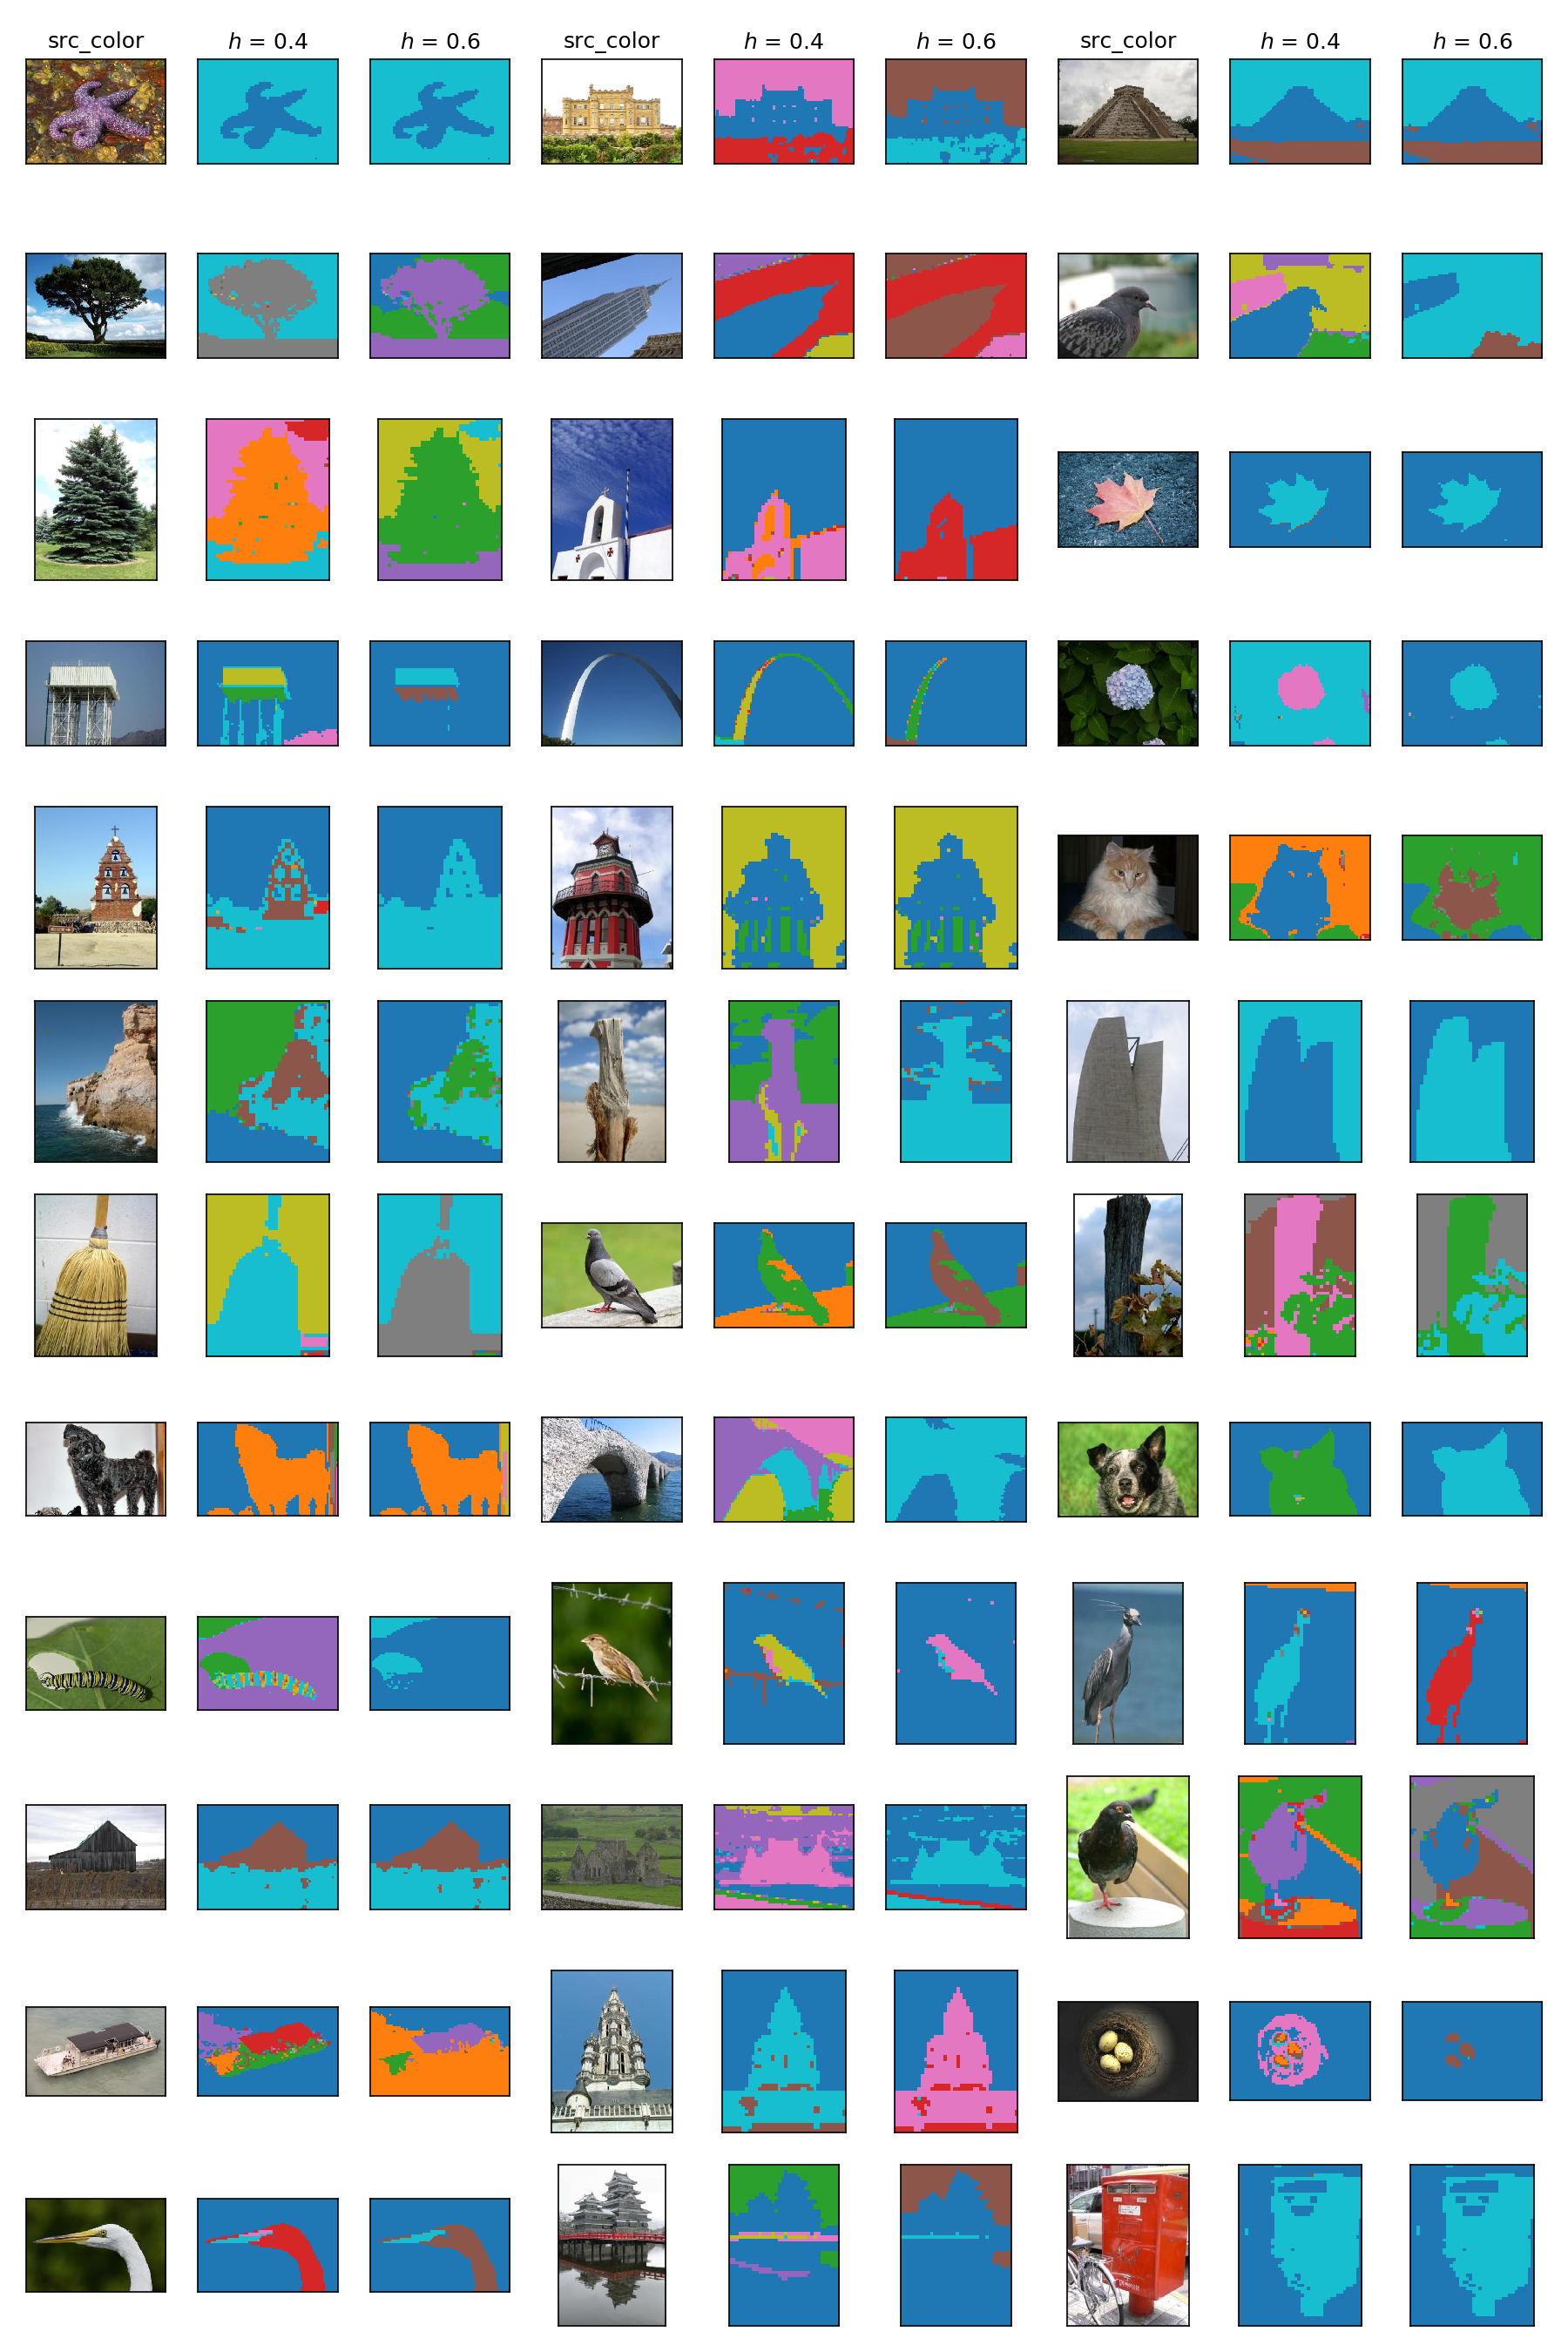
\includegraphics[width=\textwidth]{figures/segmentation-results-overview.png}
	\caption[Image segmentation results]{Image segmentation results. Author's illustration. Selected images from the ``segmentation evaluation database'' dataset. The segmentation is performed with a gaussian kernel with bandwidth 0.4 and 0.6.}
	\label{fig:segmentation-results-overview}
\end{figure}


\begin{figure}
	\centering
	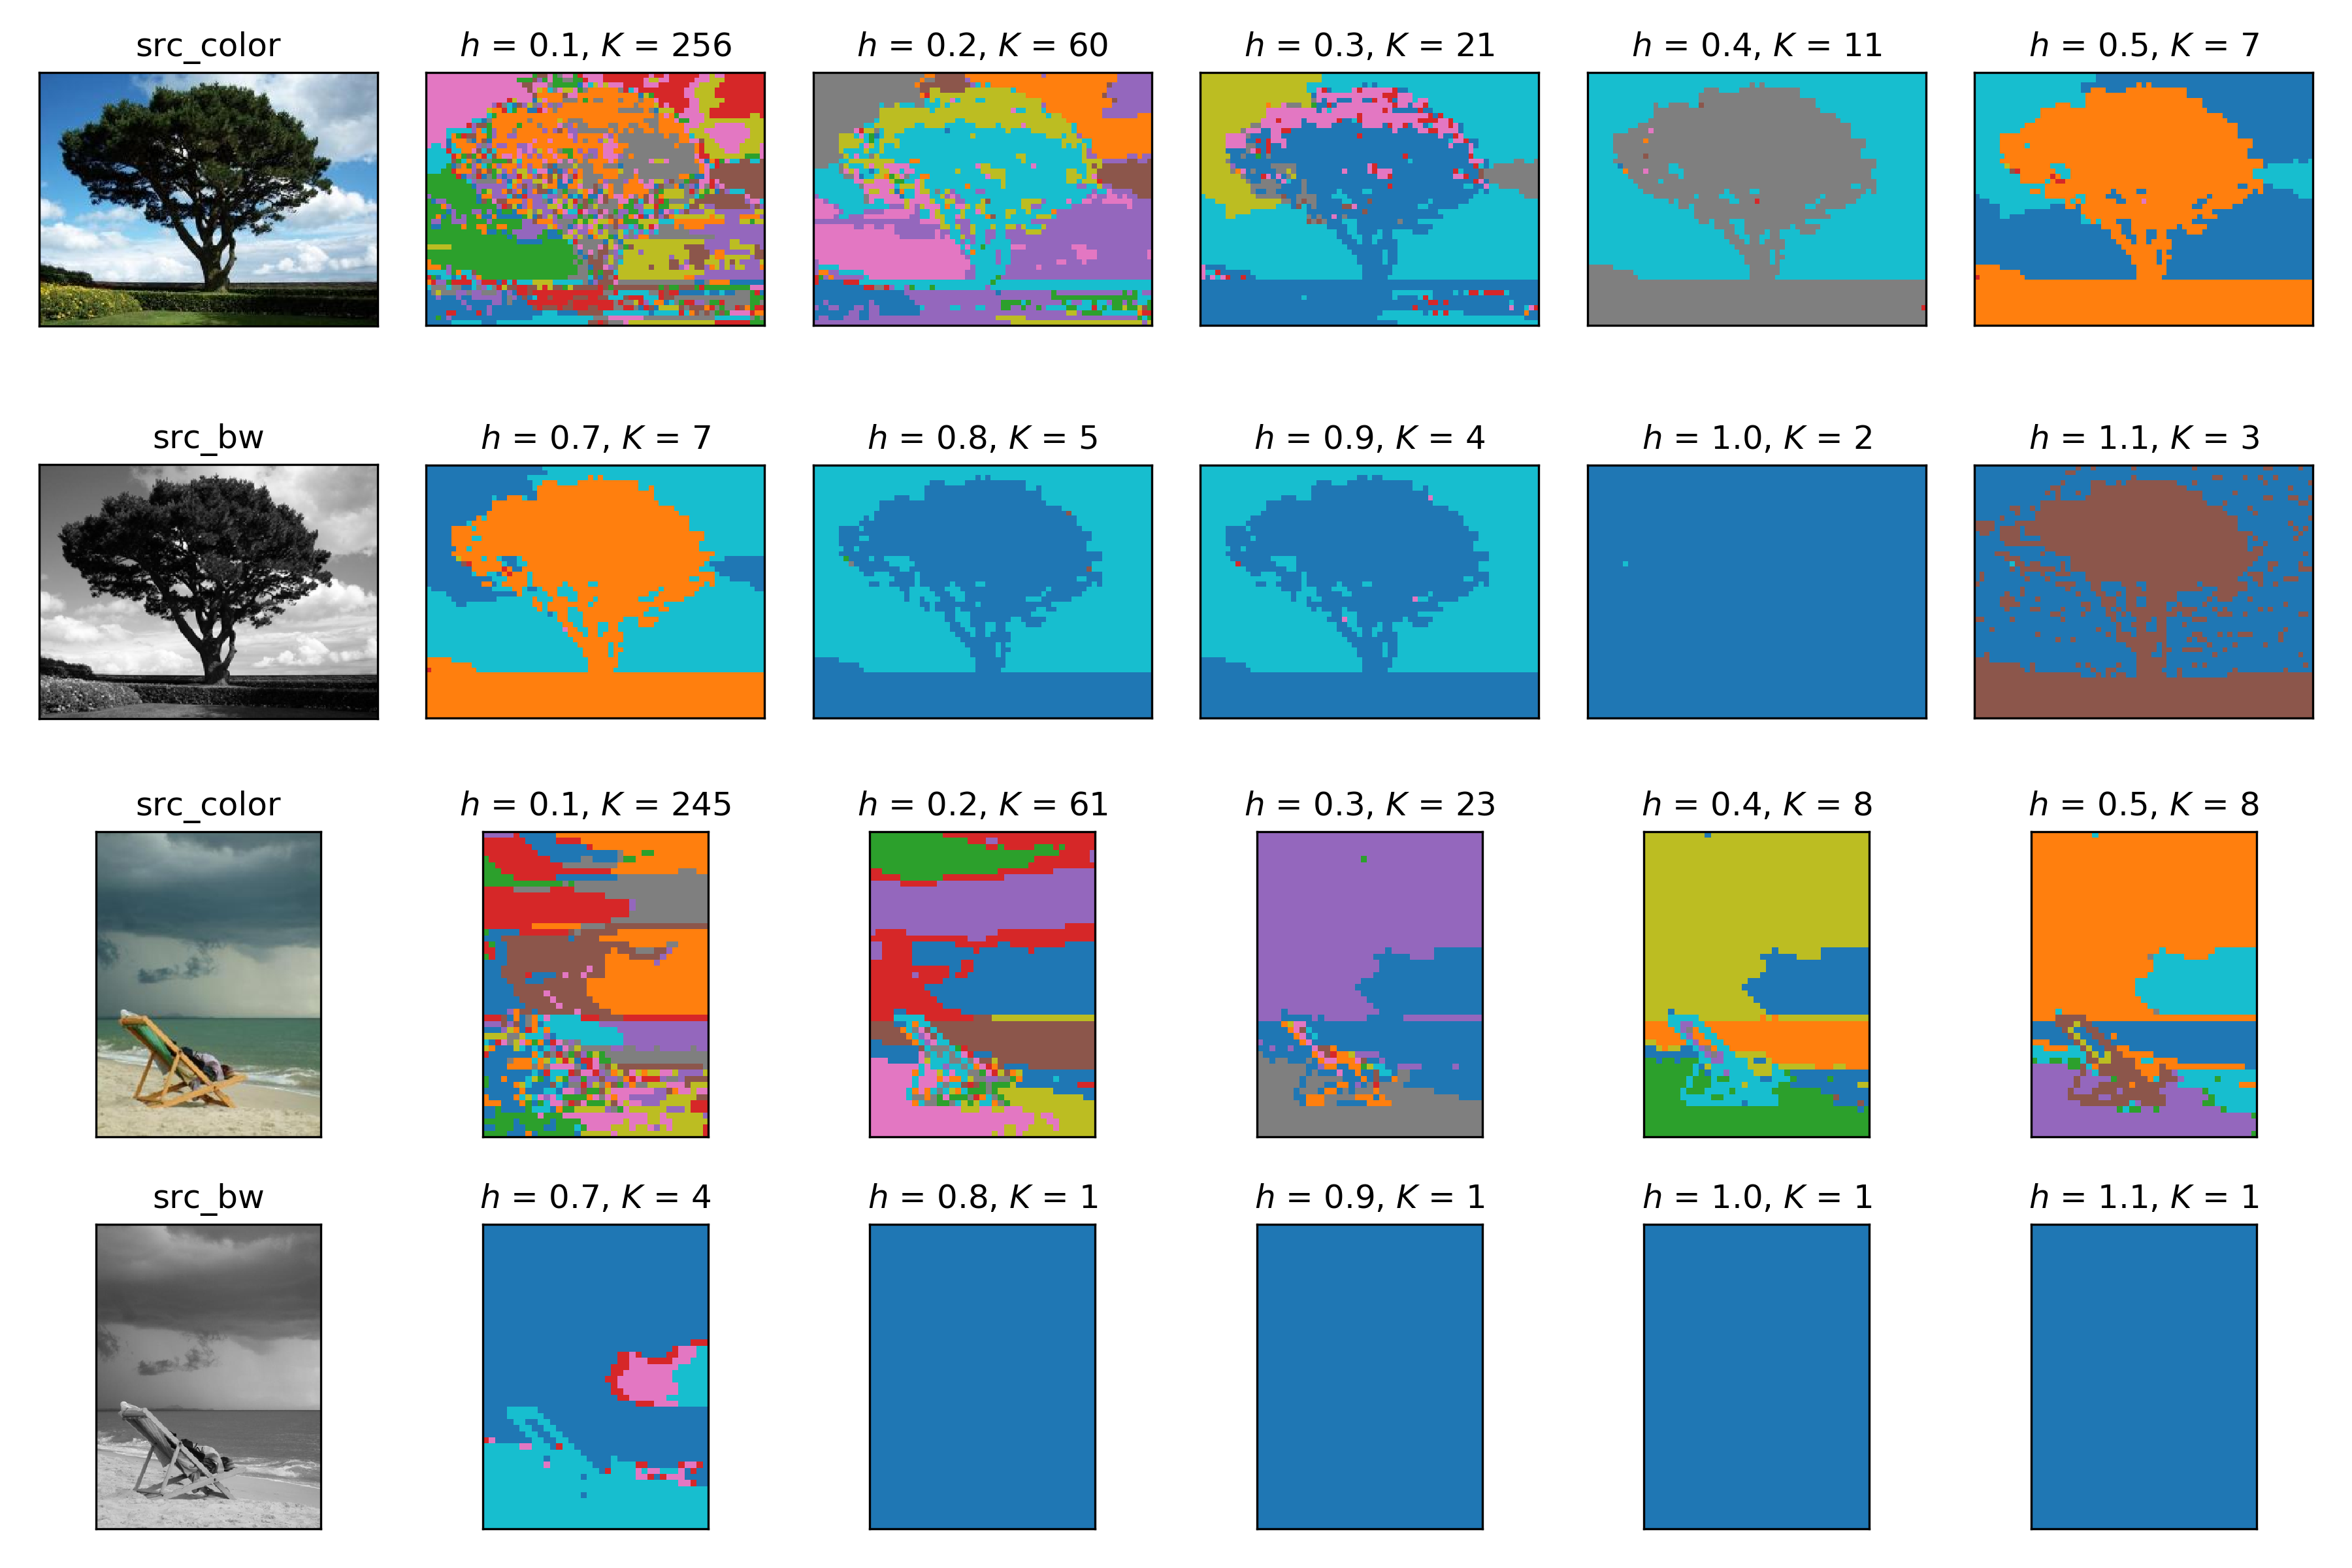
\includegraphics[width=\textwidth]{figures/segmentation-results-bandwidth-effects.png}
	\caption[Bandwidth effects]{Bandwidth effects. Author's illustration. Two images from the ``segmentation evaluation database'' dataset are segmented with the mean shift algorithm and a gaussian kernel. The color and gray scale sources are presented. Then the clustering results with varying bandwidths $h$ from 0.1 to 1.1 are plotted. The number of clusters are noted as $K$.}
	\label{fig:segmentation-results-bandwidth-effects}
\end{figure}

\begin{figure}
	\centering
	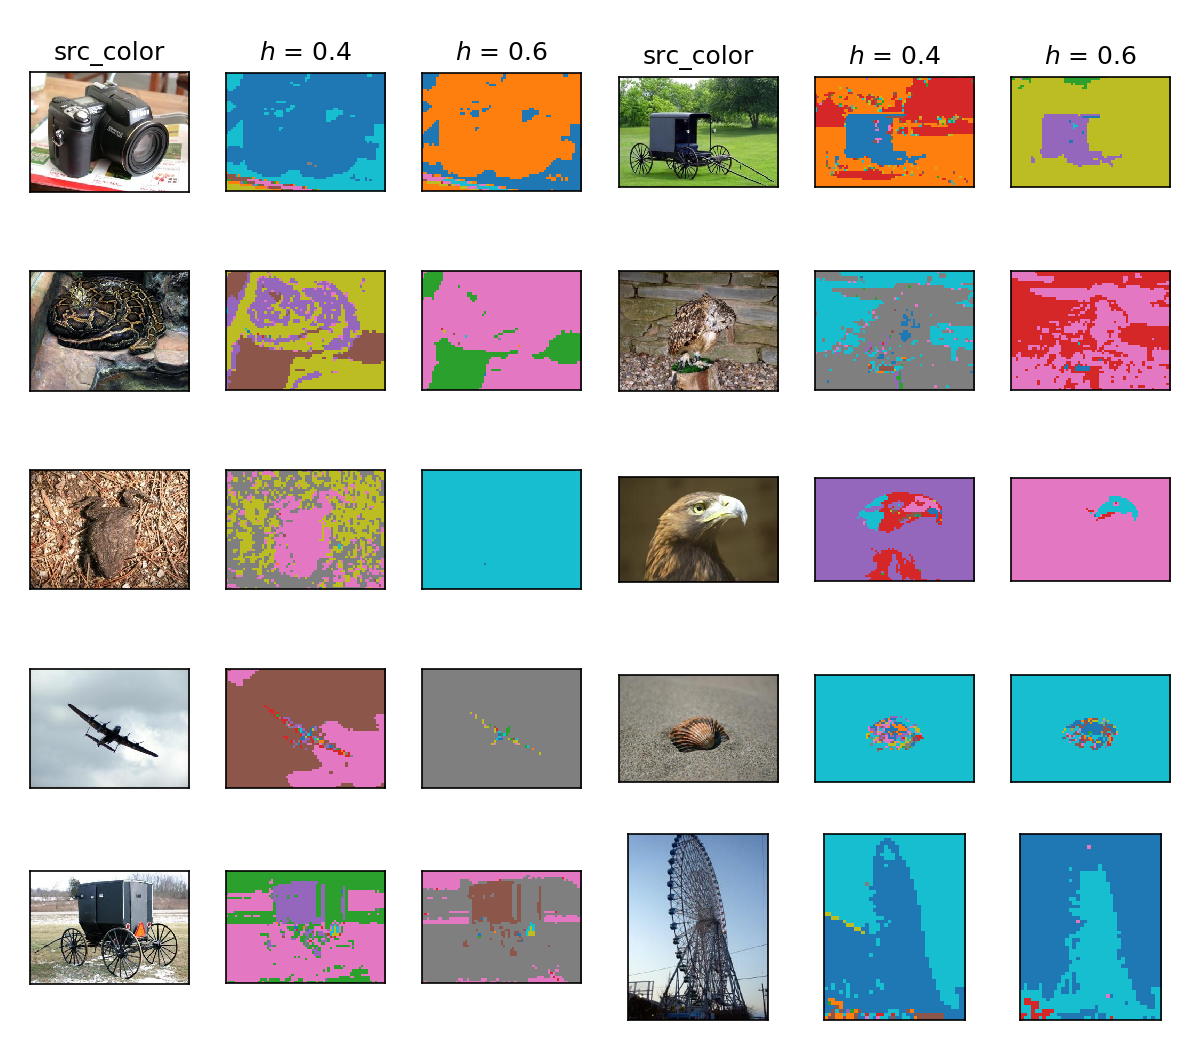
\includegraphics[width=\textwidth]{figures/segmentation-results-bad-examples.png}
	\caption[Bad image segmentation examples]{Bad image segmentation examples. Author's illustration. Selected images from the ``segmentation evaluation database'' dataset. The segmentation is performed with a gaussian kernel with bandwidth 0.4 and 0.6. These images are not well segmented by the mean shift algorithm.}
	\label{fig:segmentation-results-bad-examples}
\end{figure}


\section{Summary}

We introduced general kernel density estimates and presented popular choices for kernel functions. We derived the theory behind the mean shift algorithm and define its cluster definition. In the section \ref{sec:application} we implemented the mean shift algorithm in Matlab and applied it to an image segmentation task.

In conclusion, the mean shift algorithm is an interesting density-based clustering algorithm which is unique in its cluster definition. It has scaling problems in the dimension of the feature space. In theory the number of samples is a problem for the run time, but several speed up techniques can be implemented to effectively counter that effect. The algorithm has found its main applications in computer vision tasks but can be used as a general-purpose clustering algorithm for lower dimensional problems.


\newpage
\bibliographystyle{agsm}
\bibliography{KDEaMSC}


\appendix
\section{Code}
\begin{code}
	\lstinputlisting[language=Matlab]{../src/mean_shift.m}
	\caption[mean\_shift]{Mean shift}
	\label{code:mean_shift}
\end{code}

\begin{code}
	\lstinputlisting[language=Matlab]{../src/connected_component.m}
	\caption[connected\_component]{Connected component}
	\label{code:connected_component}
\end{code}

\begin{code}
	\lstinputlisting[language=Matlab]{../src/estimate_bandwidth.m}
	\caption[estimate\_bandwidth]{Estimate bandwidth}
	\label{code:estimate_bandwidth}
\end{code}

\begin{code}
	\lstinputlisting[language=Matlab]{../src/image_transform.m}
	\caption[image\_transform]{Image transform}
	\label{code:image_transform}
\end{code}

\newpage
\section*{Statutory Declaration}

I hereby declare, that I have written this seminar paper with the title \textbf{\thetitle} by myself and have not used other sources without declaration.


\begin{tabular}{@{}p{2in}p{2.5in}@{}}
	Karlsruhe, \thedate & \hrulefill \\
	& Jonas Spinner
\end{tabular}


\end{document}